\documentclass[12pt,twoside, letter]{exam}
\usepackage{enumitem, kantlipsum}
\usepackage[margin=1in,left=1in,right=1in,top=1in,bottom=1in]{geometry}
\usepackage{graphicx,epstopdf}
\usepackage{amssymb,amsmath,amsfonts, amsthm}
\usepackage{wasysym}
\newtheorem{theorem}{Theorem}
\newtheorem{corollary}{Corollary}[theorem]
\newtheorem{lemma}[theorem]{Lemma}
\usepackage{hyperref}
\usepackage{tikz}
\usetikzlibrary{automata, positioning}
\usetikzlibrary{matrix}
\usepackage{xstring}
\usetikzlibrary{calc}
\usepackage{ducksay}
\newtheorem{prop}{Proposition}

\theoremstyle{definition}
\newtheorem{definition}{Definition}

\usepackage{bbm}
\usepackage{verbatim}
\usepackage{bbold}
\usepackage{phfparen}
\usepackage{sets}
\newcommand{\nn}{\mathbb{N}}
\newcommand{\rr}{\mathbb{R}}
\newcommand{\cc}{\mathbb{C}}
\newcommand{\cb}{\mathcal{B}}
\newcommand{\ctau}{\mathcal{T}}
\newcommand{\co}{\mathcal{O}}
\newcommand{\zz}{\mathbb{Z}}
\newcommand{\ee}{\mathbb{E}}
\newcommand{\qq}{\mathbb{Q}}
\newcommand{\interior}{\text{Int}}
\newcommand{\pp}{\mathbb{P}}
\newcommand{\id}{\mathbbm{1}}
\newcommand{\Co}{\text{Co}}
\newcommand{\Cl}{\text{Cl}}
\usepackage{mathtools}
\DeclarePairedDelimiter\ceil{\lceil}{\rceil}
\DeclarePairedDelimiter\floor{\lfloor}{\rfloor}


\usepackage{indentfirst}
\setlist{
    listparindent = \parindent,
    parsep = 6pt,
}

\makeatletter
\newsavebox\myboxA
\newsavebox\myboxB
\newlength\mylenA

\newcommand*\xoverline[2][0.9]{%
    \sbox{\myboxA}{$\m@th#2$}%
    \setbox\myboxB\null% Phantom box
    \ht\myboxB=\ht\myboxA%
    \dp\myboxB=\dp\myboxA%
    \wd\myboxB=#1\wd\myboxA% Scale phantom
    \sbox\myboxB{$\m@th\overline{\copy\myboxB}$}%  Overlined phantom
    \setlength\mylenA{\the\wd\myboxA}%   calc width diff
    \addtolength\mylenA{-\the\wd\myboxB}%
    \ifdim\wd\myboxB<\wd\myboxA%
       \rlap{\hskip 0.5\mylenA\usebox\myboxB}{\usebox\myboxA}%
    \else
        \hskip -0.5\mylenA\rlap{\usebox\myboxA}{\hskip 0.5\mylenA\usebox\myboxB}%
    \fi}
\makeatother

\usepackage{float}
\floatstyle{boxed}
\restylefloat{figure}

\printanswers

\begin{document}


\abovedisplayskip=12pt
\belowdisplayskip=12pt
\abovedisplayshortskip=7pt
\belowdisplayshortskip=10pt
\allowdisplaybreaks

\setlength{\parindent}{18pt}

\title{Quantitative Methods: Midterm}
\author{Raymond Luo}
\date{\today}
\maketitle

\noindent {\bf Problem 1 (22 points):} We consider the Binomial tree model seen in the lectures, with 3 periods
(i.e. $N=3$) and with the parameters
\begin{equation*}
  r = 1/4, d = 1/2, u = 2
\end{equation*}
where $r$ is a simple interest rate, $d$ and $u$ respectively represent the down and up factors. Next, consider a stock price
with value $S_0 = 4$ at time $0$. We consider the price $V_n$ of a European call option, at time $n$, with payoff
\begin{equation*}
  V_3 = (S_3-5)^+
\end{equation*}
at time 3.

\begin{enumerate}
  \item Specify the risk-neutral probability weights.
    \begin{solution}
      We suppose that we are observing an arbitrage free market with a risky asset $S$ and some risk-free asset (numeraire) with interest rate $r$
      so that we know by the Fundamental Theorem of Asset Pricing that we should have a risk-neutral measure $Q$ (moreover, here it is unique) described
      by:
        \begin{align*}
          S_0 = \ee^\mathbb{Q}[S_1/(1+r)] = \frac{1}{1+r}\big[ puS_0 + (1-p)dS_0\big] \\
          \text{ where $\pp[S_1^u] = p, \pp[S_1^d] = 1-p$ define probability measure $Q$ } \\
          \Rightarrow p = \frac{S_0(1+r) - dS_0}{uS_0 - dS_0} = \frac{1 + r - d}{u - d} = \frac{1+1/4-1/2}{3/2} = \frac{1}{2}
        \end{align*}
    \end{solution}
  \item Compute the price $V_0$ of the call option at time 0.
    \begin{solution}
      We then note that the European call option as a contingent claim in an arbitrage-free extended market should also satisfy:
        \begin{align*}
          V_0 = \ee^\mathbb{Q}[V_3/(1+r)^3] \text{ where $\mathbb{Q}$ is the same risk-neutral measure as before}
        \end{align*}
        So then we have:
      $V_0 = \\
      = \frac{1}{(1+r)^3}\bigg[  {3 \choose 0}p^3(u^3S_0-K) +  {3 \choose 1}p^2(1-p)(u^2dS_0 - K) + 0 + 0 \bigg] \\
      = (\frac{4}{5})^3\bigg[\frac{1}{8}(8\cdot4 - 5) +3\frac{1}{8}(2\cdot4 - 5) \bigg] = \$2.304$
    \end{solution}
  \item Give also the delta hedging strategies $\delta_0, \delta_1,$ and $\delta_2$ at the respective times $n=0,1,2$.
    \begin{solution}\\
      The Binomial Tree of the Stock Price:\\
      \tikzstyle{bag} = [text width=2em, text centered]
      \tikzstyle{end} = []
      \begin{tikzpicture}[sloped]
         \node (a) at ( 0,0) [bag] {$\$ 4$};
         \node (b) at ( 4,-1.5) [bag] {2};
         \node (c) at ( 4,1.5) [bag] {8};
         \node (d) at ( 8,-3) [bag] {1};
         \node (e) at ( 8,0) [bag] {4};
         \node (f) at ( 8,3) [bag] {16};
         \node (g) at ( 12,-4.5) [bag] {1/2};
         \node (h) at ( 12,-1.5) [bag] {2};
         \node (i) at ( 12, 1.5) [bag] {8};
         \node (j) at ( 12, 4.5) [bag] {32};
         \draw [->] (a) to node [below] {$(1-p)$} (b);
         \draw [->] (a) to node [below] {$P$} (c);
         \draw [->] (c) to node [below] {$P^2$} (f);
         \draw [->] (c) to node [below] {$(1-p)p$} (e);
         \draw [->] (b) to node [below] {$(1-p)p$} (e);
         \draw [->] (b) to node [below] {$(1-p)^2$} (d);
         \draw [->] (f) to node [below] {$P^3$} (j);
         \draw [->] (f) to node [below] {$(1-p)p^2$} (i);
         \draw [->] (e) to node [below] {$(1-p)p^2$} (i);
         \draw [->] (e) to node [below] {$(1-p)^2p$} (h);
         \draw [->] (d) to node [below] {$(1-p)^2p$} (h);
         \draw [->] (d) to node [below] {$(1-p)^3$} (g);
      \end{tikzpicture}

      The Binomial Tree of Call Option:

      \tikzstyle{bag} = [text width=2em, text centered]
      \tikzstyle{end} = []
      \begin{tikzpicture}[sloped]
      \node (a) at ( 0,0) [bag] {$\$ 2.304$};
      \node (b) at ( 4,-1.5) [bag] {0.48};
      \node (c) at ( 4,1.5) [bag] {5.28};
      \node (d) at ( 8,-3) [bag] {0};
      \node (e) at ( 8,0) [bag] {1.2};
      \node (f) at ( 8,3) [bag] {12};
      \node (g) at ( 12,-4.5) [bag] {0};
      \node (h) at ( 12,-1.5) [bag] {0};
      \node (i) at ( 12, 1.5) [bag] {3};
      \node (j) at ( 12, 4.5) [bag] {27};
      \draw [->] (a) to node [below] {} (b);
      \draw [->] (a) to node [below] {} (c);
      \draw [->] (c) to node [below] {} (f);
      \draw [->] (c) to node [below] {} (e);
      \draw [->] (b) to node [below] {} (e);
      \draw [->] (b) to node [below] {} (d);
      \draw [->] (f) to node [below] {} (j);
      \draw [->] (f) to node [below] {} (i);
      \draw [->] (e) to node [below] {} (i);
      \draw [->] (e) to node [below] {} (h);
      \draw [->] (d) to node [below] {} (h);
      \draw [->] (d) to node [below] {} (g);
        \end{tikzpicture}

      We have the delta-hedging strategy formula by:
      $\delta_n(s) = \frac{v_{n+1}(2s)-v_{n+1}(\frac{1}{2}s)}{2s - \frac{1}{2}s}$ so that
      \begin{align*}
        \delta_0(4) = \frac{5.28 - 0.48}{8-2} = 0.8 \\
        \delta_1(8) = \frac{12 - 1.2}{16-4} = 0.9 \\
        \delta_1(2) = \frac{1.2 - 0}{4 - 1} = 0.4 \\
        \delta_2(16) = \frac{27 - 3}{32 - 8} = 1.0 \\
        \delta_2(4) = \frac{3 - 0}{8 - 2} = 0.5 \\
        \delta_2(1) = \frac{0 - 0}{2 - 0.5} = 0
      \end{align*}
    \end{solution}
  \item Consider an agent who is short 100 options. How many shares of the underlying stock does the agent hold in the hedging portfolio during
  the first time period? What is the agent's cash position at time 0? Does the agent invest in or borrow from the money
  market account to finance the hedging strategy during the first time period?
    \begin{solution}
      We note that our delta-hedging strategy formula indicates the number of shares of the underlying stock our agent would need to hold in order to hedge shorting one option,
      in the first time period. If our agent shorts 100 options, our agent holds $100\delta_0(4) = 100 \cdot 0.8 = 80$ shares of the underlying stock and invests
      his or her cash position of $100V_0 - 100\delta_0(4)\cdot S_0 = 100\cdot 2.304 - 80 \cdot 4 = -\$89.6$ in a money market account. As our agent has a negative investment
      in a money market account, the agent borrows money from a money account to finance the hedging strategy during the first time period.
    \end{solution}
\end{enumerate}


\noindent {\bf Problem 2 (15 points):}
\par{Consider the sequence of inter-arrivals times $T_1, T_2, \cdots, T_n, \cdots$ and the sequence of arrivals times $S_1, S_2, \cdots, S_n, \cdots$ of a
Poisson process $\{N(t), t \geq 0 \}$ with parameter $\lambda > 0$. Note that we have the relation}

\begin{equation*}
  S_n = \sum^{n}_{i=1} T_i
\end{equation*}

We know that $T_i$ has an exponential distribution with parameter $\lambda$, with mean $1/\lambda$ and variance $1/\lambda^2$.
\par{Show that $S_n$ is approximately normally distributed for $n$ large. Give its approximate mean and variance. }

\begin{solution}
  We note that this follows directly from the central limit theorem by observing that as $\bar{T_n} = \frac{S_n}{n}$ and the family of $\{T_{i}\}_{i \in \nn}$
  are identically and independently distributed with finite variance $1/\lambda^2$ and finite mean $1/\lambda$, by the Levy Central Limit Theorem:
    \begin{equation*}
      \sqrt{n}(\bar{T_n} - 1/\lambda) \overset{d}{\rightarrow} N(0, \sigma^2 = 1/\lambda^2).
    \end{equation*}
  It then follows that we can expect that for sufficiently large $n$, \\
  $S_{n} = n\bar{T_{n}} \approx n \cdot N(1/\lambda, 1/(\sqrt{n}\lambda)^2)$ so that $S_{n} \sim N(n/\lambda, n/\lambda^2)$
\end{solution}

\noindent {\bf Problem 3 (16 points):}
\par{Consider a sequence of independent and identically distributed random variables $X_1, X_2, \cdots, X_n, \cdots$ such that $X_i \geq 0$, with
common mean $\ee[X_{i}] = 1$. We define the sequence $M_n = \Pi^{n}_{i=1} X_i$}

\begin{enumerate}
  \item Compute $\ee[M_n]$
    \begin{solution}
      \begin{align*}
        \ee[M_n] &= \ee[\Pi^{n}_{i=1} X_i] \\
        &= \Pi^{n}_{i=1} \ee[X_i] \text{ Follows from independence} \\
        &= \Pi^{n}_{i=1} 1 = 1
      \end{align*}
    \end{solution}
  \item Consider the integers $n,p$ such that $p < n$. Show that
    \begin{equation*}
      \ee[M_n \mid \{X_k, 1 \leq k \leq p\}] = M_p
    \end{equation*}

    \begin{solution}
      \begin{align*}
        \ee[M_n \mid \{X_k, 1 \leq k \leq p\}] &= \ee[\Pi^{n}_{i=p+1} X_{i}\Pi^{p}_{j=1} X_{j} \mid \{X_k, 1 \leq k \leq p\}] \\
        &= \ee[\Pi^{n}_{i=p+1} X_{i} \mid \{X_k, 1 \leq k \leq p\}]\Pi^{p}_{j=1} X_{j} \\
        &\text{ As here $\{X_k, 1 \leq k \leq p\}$ are determined} \\
        &= \Pi^{n}_{i=p+1}\ee[ X_{i} \mid \{X_k, 1 \leq k \leq p\}]\cdot M_p \\
        &= 1 \cdot M_p = M_p
      \end{align*}
    \end{solution}
  \item Conclude.
    \begin{solution}
      Our random variable $M_n$ is a martingale.
    \end{solution}
\end{enumerate}

\noindent {\bf Problem 4 (20 points):} We consider a discrete time and discrete space Markov chain $X_n$ with state space $\{0, 1, 2, 3\}$ that
has the one-step transition probability matrix.

\begin{align*}
  \centering
    P =
  \begin{bmatrix}
    0 & 1/2 & 1/2 & 0 \\
    1/2 & 1/4 & 0 & 1/4 \\
    1/2 & 0 & 0 & 1/2 \\
    0 & 0 & 1/2 & 1/2
  \end{bmatrix}
\end{align*}
and assume that $X_0 = 0$

\begin{enumerate}
  \item Plot a diagram representing the chain
    \begin{solution}
      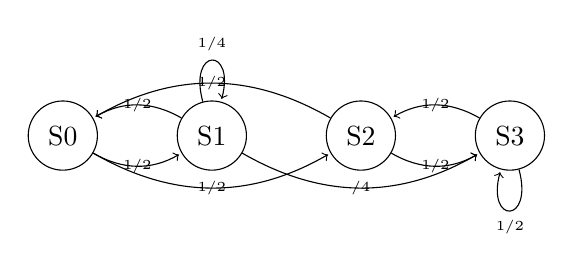
\begin{tikzpicture}
        % Draw the states
        \node[state]             (s0) {S0};
        \node[state, right=of s0] (s1) {S1};
        \node[state, right=of s1] (s2) {S2};
        \node[state, right=of s2] (s3) {S3};

        % Connect the states with arrows
        \draw[every loop]
            (s0) edge[bend right] node {{\tiny1/2}} (s1)
            (s0) edge[bend right] node {{\tiny1/2}} (s2)
            (s1) edge[bend right] node {{\tiny1/2}} (s0)
            (s1) edge[loop above] node {{\tiny1/4}} (s1)
            (s1) edge[bend right] node {{\tiny/4}} (s3)
            (s2) edge[bend right] node {{\tiny1/2}} (s0)
            (s2) edge[bend right] node {{\tiny1/2}} (s3)
            (s3) edge[bend right] node {{\tiny1/2}} (s2)
            (s3) edge[loop below] node {{\tiny1/2}} (s3);
    \end{tikzpicture}
    \end{solution}
  \item Is this Markov chain irreducible? Justify your answer
    \begin{solution}
      To show that the Markov chain is irreducible, we want to show that every state in the state space communicates with all other state spaces, i.e.
      there is a non-zero probability to reach any other state from a given state space. We note that that state 1 communicates to all other states
      (0,2,3) as there
      is a non-zero probability to transitioning to all other state spaces in one step. It then suffices to note that any state $i,j \neq 1$ can communicate
      with one another through state 1 with $i \rightarrow 3 \rightarrow j$ and $j \rightarrow 1 \rightarrow i$
    \end{solution}
  \item Compute $P^{(2)}$
    \begin{solution}
    \begin{align*}
        P^{(2)} &=
          \begin{bmatrix}
            1/2\cdot1/2+1/2\cdot1/2 & 1/2\cdot1/4 & 0 & 1/2\cdot1/4+1/2\cdot1/2 \\
            1/2\cdot1/4&1/2\cdot1/2+1/4\cdot1/4 & 1/2\cdot1/2+1/4\cdot1/4 & 1/4\cdot1/4 +1/4\cdot1/2 \\
            0 & 1/2\cdot1/2 & 1/2\cdot1/2 + 1/2\cdot1/2 & 1/2\cdot1/2 \\
            1/2\cdot1/2 & 0 & 1/2\cdot1/2 & 1/2\cdot1/2 + 1/2\cdot1/2
          \end{bmatrix}
          \\&=
          \begin{bmatrix}
            1/2 & 1/8 & 0 & 3/8 \\
            1/8 & 5/16 & 3/8 & 3/16  \\
            0 & 1/4 & 1/2 & 1/4 \\
            1/4 & 0 & 1/4 & 1/2
          \end{bmatrix}
      \end{align*}
    \end{solution}
  \item Compute $\ee[X_2 \mid X_0 = 0]$
    \begin{solution}
      $\ee[X_2 \mid X_0 = 0] =
      \begin{bmatrix}
        1 & 0 & 0 & 0
      \end{bmatrix}
      \cdot P^{(2)} \cdot
      \begin{bmatrix}
        0 \\
        1 \\
        2 \\
        3 \\
      \end{bmatrix}
      \\
      = \begin{bmatrix}
        1/2 & 1/8 & 0 & 3/8
      \end{bmatrix} \cdot
      \begin{bmatrix}
        0 \\
        1 \\
        2 \\
        3 \\
      \end{bmatrix}
      = \frac{5}{4}$.
    \end{solution}
  \item What is the probability that the chain will move to the state 2 for the first time after exactly 4 steps?
    \begin{solution}
      Note that in order for the chain to move to state 2 for the first time after exactly 4 steps, we must observe the probability of the event that
      the chain \textbf{ does not move }to state 2 at steps $n = 0, 1, 2, 3$ and transitions to state 2 on the 4th step. In order to do so, we consider modified transition matrix:
      \begin{align*}
        &P' =
        \begin{bmatrix}
          0 & 1/2 & {\bf 0} & 0 \\
          1/2 & 1/4 & {\bf 0} & 1/4 \\
          {\bf 0} & {\bf 0} & {\bf 0} & {\bf 0} \\
          0 & 0 & {\bf 0} & 1/2
        \end{bmatrix} \\
      \end{align*}
        This modification follows from the fact that we are observing the transition between states not involving state 2 for steps $n = 0, 1, 2, 3$ so we omit the transitions
        to state 2 by replacing their transition probabilities with 0 from the original matrix.
      \begin{align*}
        &\pp[\text{ first time after exactly 4 steps } \mid X_0 = 0] =
        \begin{bmatrix}
          1 & 0 & 0 & 0
        \end{bmatrix}
        \cdot (P')^{3} \cdot P\cdot
        \begin{bmatrix}
          0 \\
          0 \\
          1 \\
          0 \\
        \end{bmatrix} = \frac{5}{64}
      \end{align*}
    \end{solution}
\end{enumerate}


\noindent {\bf Problem 5 (27 points):}
\par{We consider a discrete time and discrete space Markov chain $X_n$ with state space $\{0, 1, 2, \cdots R\}$ modeling the wealth of a gambler.
The gambler starts with an initial capital equal to $i$ dollars the time $n=0$. He or she tosses a coin at each round and either gets a head with probability $p$
or gets a tail with probability $q = 1 - p$. Every time the gambler gets a head, he or she earns one dollar and every time he or she gets a tail, he or she
loses one dollar. The gambler stops playing whenever he or she is ruined, i.e. his capital $X_n$ goes down to 0 or when his or her capital reaches $R$, i.e.
$X_n = R$. We also considered the variable $M_i$, which represents the average number of rounds that must be played until the gambler goes bankrupt or reaches
a wealth equal to $R$, given an initial capital equal to $i$}


\begin{enumerate}
  \item Show that $M_0 = M_R = 0$
    \begin{solution}
      We note that by definition, we are bankrupt when we start at capital $X_0 = 0$ and we have wealth $R$ when we start at capital $X_0 = R$.
      It then follows that we don't play the game if we start at these initial positions so $M_0 = M_R = 0$.
    \end{solution}
  \item Argue that for all $i = 1, \cdots, R-1,$
    \begin{equation*}
      M_i = 1 + pM_{i+1} + qM_{i-1}
    \end{equation*}
    \begin{solution}
      Let us fix $i \in [1,R-1]$. Let $T$ be a random variable that is the number of rounds played until we either go bankrupt or reach wealth $R$. We then have that
      $M_i = \ee[T \mid X_0 = i]$
      Note that $M_i = \ee[T \mid X_0 = i] \\
      = \ee[T \mid X_0 = i \cap \text{"First coin flip is tails"}]\pp[\text{"First coin flip is tails"}] + \\
      + \ee[T \mid X_0 = i \cap \text{"First coin flip is heads"}]\pp[\text{"First coin flip is heads"}] \\
      = p\ee[T \mid X_1 = i + 1] + q\ee[T \mid X_1 = i - 1] \\
      = p( 1 + \ee[T \mid X_0 = i + 1]) + q( 1 + \ee[T \mid X_0 = i - 1]) \\
      = p + q + pM_{i+1} + qM_{i-1}\\
      = 1 + pM_{i+1} + qM_{i-1}$
    \end{solution}
  \item In this question, we choose $p = 0.5$. Show that $M_i = i(R - i)$
    \begin{solution}
      From (2), we have that $\forall i \in [1,R-1]$,
      \begin{align*}
        M_i &= 1 + pM_{i+1} + qM_{i-1} \Rightarrow \\
        \frac{1}{2} (M_{i} - M_{i-1}) &= 1 + \frac{1}{2}(M_{i+1} - M_{i}) \Rightarrow \\
        \frac{1}{2}(M_{i+1} - M_{i}) &=  \frac{1}{2} (M_{i} - M_{i-1}) - 1 = \frac{1}{2} (M_{1} - M_{0}) - i \\
      \end{align*}
      We then sum the above equation:
      \begin{align*}
        2\sum^{j-1}_{i=1}\frac{1}{2}(M_{i+1} - M_{i}) &= 2\big(\sum^{j-1}_{i=1} \frac{1}{2} (M_{1} - M_{0}) - i\big)\\
        M_{j} - M_{1} &= jM_{1} - (j-1)j \Rightarrow M_{j} = (j-1)M_{1} - j(j-1) \\
        M_{j} &= jM_{1} - j(j-1)
      \end{align*}
      It then remains for us to find $M_1$: \\
      We have that $M_{R-1} = 1 + pM_{R} + qM_{R-2} = 1 + qM_{R-2} = 1 + \frac{1}{2} M_{R-2}$. Using the above result, we have that
      \begin{align*}
        M_{R-1} &= (R-1)M_{1} - (R-1)(R-2), M_{R-2} = (R-2)M_{1} - (R-2)(R-3) \Rightarrow \\
        &2(R-1)M_{1} - 2(R-1)(R-2) - 2 = (R-2)M_{1} - (R-2)(R-3) \Rightarrow \\
        &R\cdot M_{1} = (R-2)(R+1) + 2 \Rightarrow M_{1} = \frac{(R-2)(R+1) + 2}{R}
      \end{align*}
      We then have that $M_{i} = i\frac{(R-2)(R+1)+2}{R} - i(i-1) \\
       = i\frac{R^2-R}{R} - i(i-1) = (R-1)i - (i-1)i = i(R-i)$
    \end{solution}
  \item Now, we assume that $p \neq 0.5$. Show that
    \begin{equation*}
      M_i = \frac{i}{q-p} - \frac{R}{q-p}\frac{1-(q/p)^i}{1-(q/p)^R}
    \end{equation*}
      \begin{solution}
      We start by proceeding in a similar fashion as in (3) and by noting that $p+q=1$,
      \begin{align*}
        (p+q)M_i &= 1 + pM_{i+1} + qM_{i-1} \Rightarrow \\
        q(M_{i} - M_{i-1}) &= 1 + p(M_{i+1} - M_{i}) \Rightarrow \\
        (M_{i+1} - M_{i}) &= \frac{q}{p} (M_{i} - M_{i-1}) - \frac{1}{p}  = \cdots \\
        = (\frac{q}{p})^{i} (M_{1} - M_{0}) - \sum^{i-1}_{n = 0} \frac{1}{p}(\frac{q}{p})^{n} \\
        = (\frac{q}{p})^i M_1 - \frac{1}{p}\frac{(\frac{q}{p})^i - 1}{\frac{q}{p} - 1} \\
        = (\frac{q}{p})^i M_1 - \frac{(\frac{q}{p})^i - 1}{q-p}
      \end{align*}
      We then sum the above equation:
      \begin{align*}
        \sum^{j-1}_{i=1}(M_{i+1} - M_{i}) &= \sum^{j-1}_{i=1}\bigg( (\frac{q}{p})^i M_1 - \frac{(\frac{q}{p})^i - 1}{q-p} \bigg)\\
        M_{j} &= \sum^{j-1}_{i=0} (\frac{q}{p})^i M_1 - \sum^{j-1}_{i=1} \frac{(\frac{q}{p})^i - 1}{q-p} \\
        M_{j} &= \frac{(\frac{q}{p})^j - 1}{q/p -1} M_1 - \sum^{j-1}_{i=0} \frac{(\frac{q}{p})^i}{q-p} + \frac{1}{q-p} + \frac{(j-1)}{q-p}\\
        &= M_{1}\frac{(q/p)^j - 1}{q/p -1} - \frac{1}{q-p}\bigg(\frac{(q/p)^{j}-1}{q/p-1} - j\bigg)
      \end{align*}
      It then remains for us to find $M_1$: \\
      We have that $M_{R-1} = 1 + pM_{R} + qM_{R-2} = 1 + qM_{R-2}$. Using the above result, we have that
      \begin{align*}
        M_{R-1} &= M_{1}\frac{(q/p)^{R-1} - 1}{q/p -1} - \frac{1}{q-p}\bigg(\frac{(q/p)^{R-1}-1}{q/p-1} - R + 1\bigg) \\
        % &= M_{1}\frac{(q/p)^{R-2} - 1}{q/p -1} - \frac{1}{q-p}\bigg(\frac{(q/p)^{R-1}-1}{q/p-1} - R + 1\bigg), \\
        1 + pM_{R-2} &= 1 + qM_{1}\frac{(q/p)^{R-2} - 1}{q/p -1} - \frac{q}{q-p}\bigg(\frac{(q/p)^{R-2}-1}{q/p-1} - R + 2\bigg)  \Rightarrow \\
        &M_1 \bigg(\frac{(q/p)^{R-1} - 1 - q(q/p)^{R-2} + q}{q/p - 1} \bigg) \\
        = &\frac{(q/p - q)(q/p)^{R-2}- 1 + q + (q/p-1)(-R + 1 + qR - 2q + q-p)}{(q/p - 1)(q-p)} \Rightarrow \\
        &M_1 = \frac{\big[(q/p - q)(q/p)^{R-2}-1+q\big] + \big[(q/p-1)(- R + 1 + qR - 2q + q-p)\big]}{(q-p)((q/p - q)(q/p)^{R-2}-1+q)} \\
        &= \frac{1}{q-p} + \frac{R(q - 1) + 1 - q - p}{p((q/p - q)(q/p)^{R-2}-1+q)} \\
        &\text{ [Here we use the fact that $p+q = 1$ several times]} \\
        &= \frac{1}{q-p} + \frac{-pR + 1 - 1}{p((q/p - q)(q/p)^{R-2}-p)} \\
        &= \frac{1}{q-p} + \frac{-R}{(q/p - q)(\frac{p^2}{q^2})(q/p)^{R}-p} \\
        &=  \frac{1}{q-p} + \frac{-R}{(p/q - p^2/q)(q/p)^{R}-p} \\
        &=  \frac{1}{q-p} + \frac{-R}{p[(q/p)^{R}-1]} \\
      \end{align*}
      We then have that
        \begin{align*}
          M_{i} &= \bigg(\frac{1}{q-p} + \frac{-R}{p[(q/p)^{R}-1]} \bigg)\frac{(q/p)^i - 1}{q/p -1} - \frac{1}{q-p}\bigg(\frac{(q/p)^{i}-1}{q/p-1} - i\bigg) \\
          &= \frac{i}{q-p} + \frac{-R}{p[(q/p)^{R}-1]}\frac{(q/p)^i - 1}{q/p -1} \\
          &= \frac{i}{q-p} - \frac{R}{q-p}\frac{1-(q/p)^i}{1-(q/p)^R}
        \end{align*}
      \end{solution}
\end{enumerate}

\end{document}
